%%%%%%%%%%%%%%%%%%%%%%%%%%%%%%%%%%%%%%%%%%%%%%%%%%%%%%%%%%%%%%%%%%%%%%%%%%%%%%%
% Model Staruszkiewicza
%%%%%%%%%%%%%%%%%%%%%%%%%%%%%%%%%%%%%%%%%%%%%%%%%%%%%%%%%%%%%%%%%%%%%%%%%%%%%%%
\subsection{Fundametalny relatywistyczny rotator}
Przez nierelatywistyczny rotator rozumiemy układ dwóch mas punktowych
$m_1,\ m_2$ połączonych nieważkim
prętem długości $\ell$ (rys. \ref{classic_rotator}). Lagrangian 
takiego układu w układzie środka masy ma postać~\cite{landau1978krotki}
\begin{align*}
L = \frac{m }{2} \left(\frac{\d r}{\d t}\right)^2, 
\quad m=m_1+m_2, r=r_2-r_1
\end{align*}
gdzie $r_1,\ r_2$ to odpowiednio położenia mas $m_1$, $m_2$.
Zauważmy, że $||r|| =\ell = const$, a zatem interesuje nas jedynie kierunek 
wyznaczony przez $r$.
Wersor $ \hat{r} = r / \ell$ możemy przedstawić za pomocą  
współrzędnych sferycznych
\begin{align*}
\hat{r} = ( \cos \phi \sin\theta, \ \sin\phi\sin\theta,\ \cos\theta )
\end{align*}
Obracamy układ odniesienia tak, aby $\theta = \pi/2$. Lagrangian 
przyjmuje wtedy postać
\begin{align*}
L = \frac{m\ell^2 }{2} \left(\frac{\d \phi}{\d t}\right)^2
\end{align*}
Z równania Eulera-Lagrange'a dla $\phi$ wynika, że 
\begin{align*}
\ddot{\phi} = 0
\end{align*}
A zatem $\phi \sim t$, to znaczy, że 
nierelatywistyczny rotator mierzy Newtonowski czas
absolutny $t$. Skłania nas to do refleksji nad możliwością 
wykorzystania relatywistycznego rotatora 
do pomiarów czasu. Prostota układu sugeruje, że 
może on być odpowiedni do testowania hipotezy zegara.
\begin{figure}
\centering
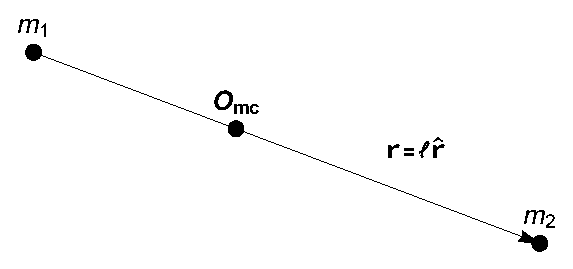
\includegraphics[scale=0.6]{classic_rotator2.eps}
\caption{Klasyczny rotator składający się z dwóch mas $m_1$, $m_2$ 
połączonych nieważkim prętem długości $\ell$.}
\label{classic_rotator}
\end{figure}

Przeniesienie tego układu na grunt relatywistyczny wprowadził 
profesor Staruszkiewicz~\cite{star2008} proponując następujące 
definicje:
\begin{definition}
Relatywistyczny rotator to układ dynamiczny
 opisany przez położenie $x$ i kierunek
zerowy $k$ oraz dodatkowo dwa parametry: masę $m$ i długość $\ell$.
\end{definition}
\begin{definition}
Układ dynamiczny  nazywamy fenomenologicznym jeżeli jego niezmienniki Casimira są 
całkami ruchu. Układ dynamiczny nazywamy fundamentalnym jeżeli jego niezmienniki
Casimira są parametrami (m. in. nie zależą od warunków początkowych).
\end{definition}
Powtórzymy teraz konstrukcję przedstawioną we wspomnianej pracy oraz w
~\cite{Kassandrov2009, Bratek2009nonuniq}.
W oparciu o powyższe definicje można skonstruować fundamentalny
relatywistyczny rotator. Z wielkości zawartych w definicji relatywistycznego 
rotatora możemy utworzyć bezwymiarową wielkość
\begin{align*}
\xi = - \ell^2 \frac{\dot{k} \cdot \dot{k}}{ ( k \cdot \dot{x})^2 }.
\end{align*}
Możemy wtedy utworzyć Lagrangian postaci
\begin{align}\label{rotatorStar}
L = m \sqrt{ \dot{x} \cdot \dot{x} } f( \xi ) .
\end{align}
%Więz $k\cdot k= 0$ możemy uwzględnić wprowadzając mnożnik Lagranga $\lambda$
%\begin{align}
%L = m \sqrt{ \dot{x} \cdot \dot{x} } f( \xi ) + \lambda( k\cdot k ).
%\end{align}a
%Wtedy równanie Eulera-Lagranga dla $\lambda$ daje odpowiedni więz.
Działanie związane z powyższym Lagrangianem 
jest niezmiennicze ze względu reparametryzację, 
Lorenzowsko niezmiennicze. Dodatkowo $k$ wskazuje kierunek zerowy, a zatem
 układ fizyczny nie zmienia się
po przeskalowaniu $k \to a k$. 
Nie jest to najogólniejszy relatywistyczny 
rotator jaki można wziąć pod uwagę, gdyż $\xi$ nie jest jedyną 
możliwą bezwymiarową kombinacją wielkości charakterystycznych 
dla relatywistycznego rotatora~\cite{Bratek2009nonuniq}.


Oznaczamy przez $P_\mu$ i $\Pi_\mu$ pędy kanoniczne związane 
odpowiednio z $x$ i $k$ oraz przez $M_{\mu\nu}$ całkowity moment pędu.
\begin{align*}
P_\mu &= \frac{\partial L}{\partial \dot{x}^\mu}, \qquad
\Pi_\mu = \frac{\partial L}{\partial \dot{k}^\mu} \\
M_{\mu\nu} &= x_\mu P_\nu - P_\mu x_\nu + k_\mu \Pi_\nu - \Pi_\mu k_\nu.
\end{align*}

Dla Lagrangianu~\ref{rotatorStar} mamy 
\begin{align*}
P_\mu &=  \frac{m}{\sqrt{ \dot{x} \cdot \dot{x} }} f(\xi) \dot{x}_\mu 
- 2 \frac{m}{k \cdot \dot{x}} \sqrt{ \dot{x} \cdot \dot{x} }
f'(\xi) \xi k_\mu  \\
\Pi_\mu &= 2 \frac{m}{\dot{k} \cdot \dot{k}} \sqrt{ \dot{x} \cdot \dot{x} }
f'(\xi) \xi \dot{k}_\mu
\end{align*}

Niezmiennikami Casimira będą w tym przypadku $P_\mu P^\mu$ oraz
$W_\mu W^\mu$ gdzie $W$ jest pseudowektorem Pauliego-Lubańskiego 
danym przez
\begin{align*}
W_\mu = - \frac{1}{2} \varepsilon_{\mu\nu\rho\sigma}
M^{\nu\rho} P^\sigma
\end{align*}

Kontrakcja tensora antysymetrycznego $A_{\mu\nu}$ z 
tensorem symetrycznym $S_{\mu\nu}$ jest równa zeru. 
Korzystając z tego i antysymetrii tensora $\varepsilon$ dostajemy
\begin{align*}
W_\mu = - \frac{1}{2} \varepsilon_{\mu\nu\rho\sigma}
(x^\mu P^\nu - P^\mu x^\nu + k^\mu \Pi^\nu - \Pi^\mu k^\nu) P^\sigma = 
 - \frac{1}{2} \varepsilon_{\mu\nu\rho\sigma}
( k^\mu \Pi^\nu - \Pi^\mu k^\nu) P^\sigma = 
  \varepsilon_{\mu\nu\rho\sigma}
 \Pi^\mu k^\nu P^\sigma
\end{align*}
Dla Lagrangianu~\ref{rotatorStar} możemy zapisać $W_\mu$ w postaci
\begin{align*}
W_\mu =  \varepsilon_{\mu\nu\rho\sigma}  \Pi^\mu k^\nu P^\sigma =
2\frac{m^2}{ \dot{k} \cdot \dot{k}} 
f(\xi) f'(\xi) \xi \varepsilon_{\mu\nu\rho\sigma} 
 \dot{k}^\mu k^\nu \dot{x}^\sigma
\end{align*}
Pozwala to zapisać $W_\mu W^\mu$ w postaci wyznacznika Gramma
\begin{align*}
W_\mu W^\mu = 
4 \frac{m^4}{ (\dot{k} \cdot \dot{k})^2} 
f(\xi)^2 f'(\xi)^2 \xi^2 
\left| 
\begin{array}{ccc}
\dot{k} \cdot \dot{k}& \dot{k} \cdot k& \dot{k} \cdot \dot{x}\\
k \cdot \dot{k}& k \cdot k &k  \cdot \dot{x}\\
\dot{x} \cdot \dot{k}& \dot{x} \cdot k &\dot{x} \cdot \dot{x}
\end{array}
\right|
\end{align*}
Inwestując równości $k\cdot k=0$, $\dot{x}\cdot\dot{x}$ 
oraz $\dot{k} \cdot k= 0$ dostajemy
\begin{align*}
P_\mu P^\mu =  m^2( f(\xi)^2- 4 f(\xi) f'(\xi) \xi)
W_\mu W^\mu = 
 - 4 m^4\ell^2  f(\xi)^2 f'(\xi)^2 \xi
\end{align*}
Zakładamy, że rotator jest fundamentalny, a więc niezmienniki
Casimira powinny być parametrami, co można zapisać w postaci
równości
\begin{align} \label{casimir1}
P_\mu P^\mu = m^2 \tag{C1}
\end{align}
\begin{align} \label{casimir2}
W_\mu W^\mu = - \frac{1}{4} m^4 \ell^2\tag{C2}
\end{align}
\begin{align*} 
 f(\xi)^2- 4 f(\xi) f'(\xi) \xi
\stackrel{\text{\ref{casimir1}}}{=} 
1 \stackrel{\text{\ref{casimir2}}}{=}
  16   f(\xi)^2 f'(\xi)^2 \xi
\end{align*}
Powyższe rozwiązanie mają wspólne rozwiązanie 
postaci (zobacz dod. A)
\begin{align*}
f(\xi ) = \pm \sqrt{ 1 \pm \sqrt{\xi} }.
\end{align*}
Z fizycznych powodów wybieramy znaki $+$~\cite{Bratek2009nonuniq}.
\begin{align*}
f(\xi ) =  \sqrt{ 1 + \sqrt{\xi} }.
\end{align*}

To że dwa równania różniczkowe miały wspólne rozwiązanie 
wydaje się być szczęśliwym zbiegiem okoliczności. 
Niestety otrzymany Lagrangian ma defekt i ruch takiego 
rotatora nie jest deterministyczny~\cite{Bratek2012Spinorindeterm}.
Przedstawimy teraz uogólnienie takiego rotatora,
które możemy znaleźć w~\cite{Bratek2015wiele}.


